\documentclass[border=2pt]{standalone}

% --- UNIVERSAL PREAMBLE BLOCK ---

% Graphics and Plots
\usepackage{tikz}
\usepackage{pgfplots}
\pgfplotsset{compat=1.18}
\usetikzlibrary{calc, patterns, positioning, shapes.geometric}

% Define Colors
\definecolor{Garnet}{HTML}{73000A}
\definecolor{Gray70}{gray}{0.70}
\definecolor{SoftGray}{gray}{0.95}

% Global PGFPlots settings
\pgfplotsset{
    every axis/.style={
        axis line style={draw=black, line width=0.8pt},
        tick style={draw=black, line width=0.6pt},
        tick label style={font=\scriptsize\color{black}},
        label style={font=\footnotesize\bfseries\color{black}},
        grid=major,
        grid style={draw=Gray70, line width=0.2pt, dashed},
        legend style={
            draw=black,
            fill=white,
            font=\tiny,
            cells={anchor=west}
        },
        ybar,
        bar width=12pt,
        ymin=0,
        enlarge y limits={upper=0.1},
    },
    barstyle/.style={
        draw=black,
        fill=Garnet,
        fill opacity=0.7,
        line width=0.6pt,
        text opacity=1
    }
}

\begin{document}

    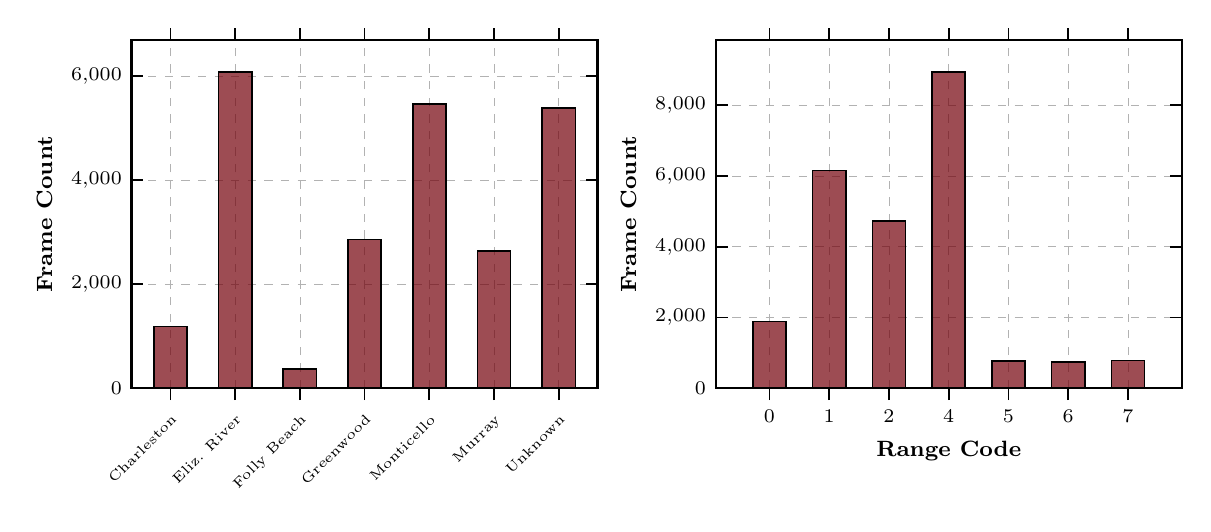
\begin{tikzpicture}

        % --- CHART 1
        \begin{axis}[
            name=plot1,
            width=7.5cm, height=6cm,
            symbolic x coords={Charleston, Eliz. River, Folly Beach, Greenwood, Monticello, Murray, Unknown},
            xtick=data,
            xticklabel style={
                rotate=45,
                anchor=north east,
                font=\tiny
            },
            ylabel={Frame Count},
            % xlabel={Location}, % Removed as requested
            enlarge x limits=0.1
        ]
            \addplot[barstyle] coordinates {
                (Charleston,1185)
                (Eliz. River,6081)
                (Folly Beach,367)
                (Greenwood,2862)
                (Monticello,5462)
                (Murray,2641)
                (Unknown,5393)
            };
        \end{axis}

        % --- CHART 2:
        \begin{axis}[
            name=plot2,
            at={(plot1.north east)},
            anchor=north west,
            xshift=1.5cm,
            width=7.5cm, height=6cm,
            symbolic x coords={0,1,2,4,5,6,7},
            xtick=data,
            ylabel={Frame Count},
            xlabel={Range Code},
            enlarge x limits=0.15
        ]
            \addplot[barstyle] coordinates {
                (0,1884)
                (1,6151)
                (2,4732)
                (4,8938)
                (5,768)
                (6,734)
                (7,784)
            };
        \end{axis}

    \end{tikzpicture}

\end{document}